\section{Introduction}
\label{sec:introduction}

\newcommand{\introfigleftvoffset}{-3cm}

\begin{wrapfigure}[12]{r}{0.3\textwidth}
  \hspace*{0.6em}\begin{minipage}{\dimexpr\linewidth-1em}
    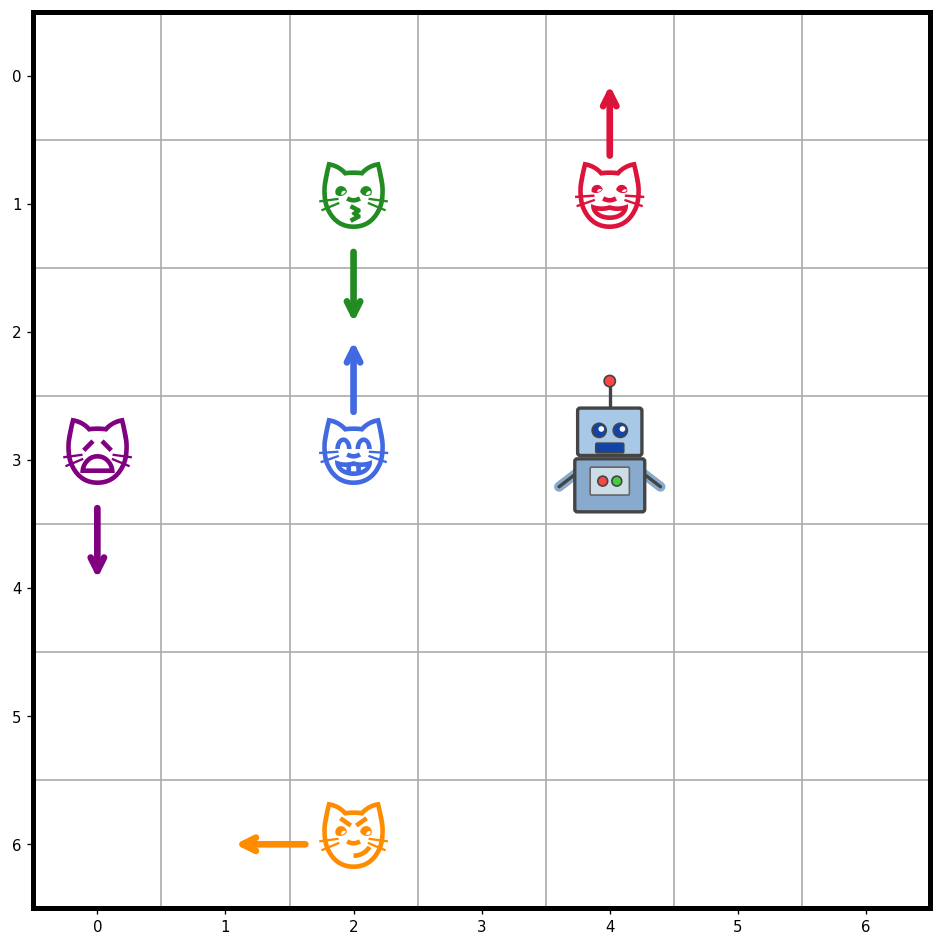
\includegraphics[width=\linewidth]{img/grid_preview.png}
    \caption{Cat Feeder env.}
    \label{fig:grid_preview_intro}
  \end{minipage}
\end{wrapfigure}
Consider the problem of controlling a mobile robot deployed in a cat shelter whose task is to deliver food to cats roaming around the facility (Figure~\ref{fig:grid_preview_intro}). 
New food requests from hungry cats may arrive at arbitrary times and locations, while existing requests may disappear if a cat wanders away before being served.
Since the robot can serve only one cat at a time, fulfilling one request may delay others, potentially allowing some cats to move farther away. 
Thus, the robot must dynamically adapt to the set of active requests to maximize the number of cats fed before they disappear.

In this work, we model the above control problem as a multi-objective reinforcement learning task in which all the objectives come from an identical family, such as reachability in this case.
These objectives can be conflicting and any number of them may be active at a given time.
Moreover, we make no assumptions about their distribution or arrival pattern.
Our goal is to design adaptive policies that update their behavior seamlessly as objectives appear or disappear.

The class of problems we study is relevant to many real-world scenarios.
For example, a warehouse robot must be responsive to changing pickup, delivery, and sorting tasks, and this setting has motivated work on warehouse robot path planning and resource allocation~\citep{chen2023warehouserobot,shen2023amazonrobotics}.
More broadly, such problems have been extensively studied in the planning literature~\citep{fox2006plan}, typically assuming that a precise environment model (like a graph) is available without uncertainties. 
Existing reinforcement learning-based path planning methods~\citep{singh2023reviewrlpathplanning} are able to handle uncertainties but cannot adapt to varying number of objectives at deploying time.
% In contrast, within reinforcement learning (RL) settings---where the environment may be uncertain and a model may not be available---this problem has not been studied to the best of our knowledge.

To solve this problem, we propose a novel compositional RL framework, where each objective is served using a local policy, selfishly maximizing its assigned objective by competing against the other policies.
Coordination between these policies is achieved through a novel auction-based mechanism:
at every decision step, policies submit bids for the right to execute their actions, where bids reflect the urgency of the current state with respect to their objectives. 
The highest bidder selects the action, enabling a dynamic and interpretable trade-off among objectives.
Returning to the cat feeder example, suppose the robot approaches an intersection with two active requests, the policy for the first request recommends turning left, while the policy for the second recommends turning right. 
Since both actions cannot be executed simultaneously, a trade-off is unavoidable. 
The auction mechanism determines which objective is prioritized, based on the relative urgency encoded in the bids.

This compositional design yields strong modularity, facilitating fast adaptation:
when an objective appears or disappears, only the corresponding policy needs to be added or removed.
Furthermore, when objectives belong to the identical family---which is reachability in our case---a single generalized policy can be trained for the entire family. 
We can deploy identical \emph{copies} of this policy when new objectives arrive, enabling immediate adaptation. 
Modularity also permits us to define objective-specific reward signals while the auction mechanism takes care of the trade-offs between objectives.
For example, we can easily define a distance-based dense reward signal for each policy controlling the cat feeder to move closer to its assigned cat.
In contrast, it is challenging to define such a dense reward signal to train a monolithic policy to trade-off between the multiple objectives.
% We have to resort to imposing a preference ordering over the multi-dimensional reward vector, or stick to sparse rewards.
% In contrast, a monolithic policy serving multiple objectives would require additional machinery to impose a dense preference ordering over the multi-dimensional reward vector, which is typically complex and often subject to debate.
We show in our experiments that monolithic policies, trained with both sparse rewards and different types of scalarized dense rewards, fall much short of the payoffs achieved by our modular approach.

Yet another advantage of our modular framework is interpretability.
At any moment, we can determine the policy in control, and thereby the objective currently being pursued by the agent. 
This explanation is beneficial in a range of real-world situations, like providing post-hoc explanations of failures, and also feedback on biases in pursuing different objectives.

We implement our modular framework as a general-sum game between local policies seeking to fulfill their assigned objectives, and this game is set up using a simple wrapper around existing multi-objective environments. 
Each agent's action space is augmented with an additional numeric variable representing the bids, and the transitions between the game's states encode the execution of the action selected by the highest bidder.
However, we still need to address some challenges.

\textbf{Challenge I: Enforcing honest bids.}
While the auction mechanism treats all policies fairly, the policies must still place honest bid in proportion to their urgency. 
Otherwise, they may learn to overbid and suppress competitors, resulting in suboptimal results. 
To prevent this, we impose penalties during training that scale with the bid values. 
As a consequence, excessive bidding reduces the net return of a policy, thus aligning its incentives with truthful urgency estimation---a policy only bids high when it is sure to receive a reward (when it feeds the cat) or to avoid a penalty (when a cat is close to disappearing).
Our theoretical results formalize this intuition by showing that, when one objective is sufficiently more urgent than the others, the auction selects the corresponding policy.

\textbf{Challenge II: Achieving environment awareness.}
Effective bidding depends not only on the current state and the local objective, but also on the configuration of competing objectives. 
For instance, in the cat feeder problem, if two requests are spatially close, their policies need not compete aggressively. 
Conversely, if requests lie in opposite directions, the urgent policy must bid sufficiently high to win. 
To enable such environment-aware bidding, we allow the policies to observe all the objectives, i.e., the policies have information about the global state. 
But a large number of objectives makes the global state vector very big, and so the policies use an \textit{attention pooling} architecture that can extract relevant information from the active objectives into an embedding vector.
This module also enables policies to process varying number of objectives at deployment time.
% Additionally, the policies are trained concurrently so that they learn to optimize payoffs in the presence of opponents.

\textbf{Challenge III: Unbounded objective count.}
When policies have to compete with many objectives, providing each with the global state results in a very high dimensional observation space.
This makes training slow with a standard neural network policy.
We address this with an attention pooling mechanism that aggregates information about an arbitrary number of competing objectives into a fixed-dimensional representation. 
Each local policy is equipped with its own pooling module which is co-trained with the policy.
This architecture also lets policies operate with more objectives at test time than were present during training, because the pooling module maps any number of objective states to a fixed-size representation.

% During deployment, there may be more active objectives than during training. 
% This invalidates standard game-theoretic training formulations which assume a fixed number of opponents. 

We test our framework on three environments with dynamic reachability objectives: the cat feeder environment implemented as a gridworld, and two Atari games: Assault and Air-raid~\citep{bellemare13arcade}.
We use proximal policy optimization (PPO; \citet{schulman2017ppo}) to train our policies by running one instance of PPO for each policy while they compete against each other.
We observe empirical convergence of training and substantially better or equal performance compared to baselines in the three environments.
By deploying copies of trained policies, we demonstrate the ability of our method to generalize to more objectives at test-time than during training.
Lastly, to aid interpretability in renderings of rollouts, we implement visualization of the policy in control and the objective being pursued, using which we empirically observe strategic bidding behaviors between policies.

In summary, our contributions consist of the following:
\begin{enumerate}
  \item We formulate an auction-based modular framework for multi-objective RL that consists of objective-specific local policies competing with each other through auctions. Also, theoretical guarantees for urgency-based policy selection are established in~\Cref{sec:auction-framework}.
  \item We introduce a multi-policy architecture that can handle varying numbers of objectives, and provide a PPO-based training procedure in~\Cref{sec:learning-local-policies}.
  \item We evaluate the method on three multi-objective environments comparing against baselines in~\Cref{sec:experimental-results} and demonstrate the superior performance of our policies.
\end{enumerate}
